\documentclass[dvipdfmx, dvipsnames]{beamer}
\usetheme[secheader]{Boadilla}
% \usepackage{beamerthemesplit} // Activate for custom appearanced
%\setbeamertemplate{caption}[numbered]
\usefonttheme[onlymath]{serif} %数式をゴシックにしない
%\setbeamertemplate{blocks}[rounded] % Blockの影を消す
\useinnertheme{circles} % 箇条書きをシンプルに
\setbeamertemplate{navigation symbols}{} % ナビゲーションシンボルを消す
\setbeamertemplate{footline}[frame number] % フッターはスライド番号のみ
\setbeamercolor{page number in head/foot}{fg=black}
% \usepackage{beamerthemesplit} // Activate for custom appearance
%\setlength{\parindent}{1em}  %段落字下げ
\renewcommand{\figurename}{Fig}
\renewcommand{\tablename}{Tab}
\usepackage[caption=false]{subfig}
\usepackage{amsmath}
%\usepackage{blindtext}
\usepackage{tikz}
\usetikzlibrary{matrix, shapes, backgrounds, positioning, decorations.pathreplacing,calligraphy}
\usetikzlibrary{angles,quotes} % for pic
\usepackage{tcolorbox}
 \tcbuselibrary{theorems,skins} 
\setbeamerfont{itemize/enumerate subbody}{size=\normalsize} %subitem を同じ大きさに
%
%\setbeamertemplate{itemize subitem}{\normalsize\raise1.25pt\hbox{\donotcoloroutermaths$\blacktriangleright$}}  %to set the symbol size
\usepackage{caption}
\usepackage{fancyvrb}
\usepackage{algorithm}
\usepackage{algpseudocode}
\usepackage{appendixnumberbeamer}
%数式用の下線
\def\mathunderline#1#2{\color{#1}\underline{{\color{black}#2}}\color{black}}

\setbeamercolor{block title}{bg=gray!10} %block title の背景
\setbeamercolor{block body}{bg=white} %block の中身

%list を black-right-triangle にするコマンド
\newcommand{\triangleitem}{
\setbeamertemplate{itemize item}{\color{RedOrange}$\blacktriangleright$}
\setbeamertemplate{itemize subitem}{\color{RedOrange}$\blacktriangleright$}
}

\title{大規模な疎行列に適した確率的主成分分析の計算法とその拡張}
\date{2026年6月13日}

%\renewcommand*{\thefootnote}{\fnsymbol{footnote}}
%\setcounter{footnote}{0} 

\author {阿部興\footnote{東京科学大学 総合研究院 難治疾患研究所} (発表者)  ・島村徹平$^1$}

\begin{document}
\frame{
\titlepage
}

\begin{frame}
\frametitle{動機: 事例}

\vfill

細胞ごとに遺伝子の発現量を計測できる \structure{単一細胞 RNA-seq} は疾患の機序を解明するための豊富な情報を持つ.

\vfill

しかし高次元で0が多い(疎;sparse)

\vfill

\begin{figure}
\includegraphics[height=0.3\textheight, clip]{./img/heatmap.png}
\caption{ゼロ要素を白, 非ゼロ要素を黒としたヒートマップ. 黒はほとんど見えない.各行は遺伝子,各列は細胞. Bischoff et al. (2021)\footnotemark[1]. }
\end{figure}

\footnotetext[1]{Bischoff, P., Trinks, A., Obermayer, B. et al. Single-cell RNA sequencing reveals distinct tumor microenvironmental patterns in lung adenocarcinoma. Oncogene 40, 6748–6758 (2021). \url{https://doi.org/10.1038/s41388-021-02054-3}}
\end{frame}

\begin{frame}
\frametitle{動機: 精神面}
\begin{figure}
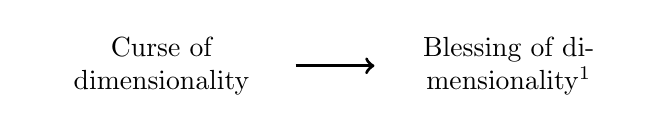
\begin{tikzpicture}[every node/.style={text width=90pt, align=center}]
\node at (0,0)(curse){Curse of\\ dimensionality};
\node[right = of curse](bless){Blessing of dimensionality\footnotemark[1]};
\path[draw, very thick, ->](curse)--(bless);
\end{tikzpicture}
\end{figure}
\begin{columns}
\begin{column}{0.5\textwidth}
\begin{itemize}
\item[$\bigcirc$] 高次元の積分は難しい
\item[$\triangle$] 高次元のデータはややこしい
\end{itemize}
\end{column}
\begin{column}{0.5\textwidth}
\begin{itemize}
\item[$\circledcirc$] 見えるものが多いとうれしい \color{gray}{たとえそのほとんどが ``0" だとしても}
\end{itemize}
\end{column}
\end{columns}

\vfill 

大規模で疎なデータを活用するためには…
\begin{itemize}
\item 計算効率を高める
\item 背景知識の活用
\end{itemize}

\footnotetext[1]{Gelman, A. (2004).``The blessing of dimensionality'' \url{https://statmodeling.stat.columbia.edu/2004/10/27/the_blessing_of/}}
\end{frame}

\begin{frame}
\frametitle{主成分分析}

\begin{align*}
\underbrace{Y}_{D_1 \times D_2} \approx \underbrace{V^{(1)}}_{D_1 \times L} \underbrace{ \{ V^{(2)} \}^\top } _{L \times D_2}
\end{align*}

他の分析の入力としても使われる
\end{frame}

\begin{frame} 
\frametitle{疎行列の形式}

Coordinate (COO) 形式:

行列 $Y$ の $(i,j)$ 成分 $y_{ij}$ を $ \mathcal{D}_n = (\boldsymbol{x}_n, y_n)= ((x_{n1}, x_{n2}),y_{n})= ((i, j),y_{ij})$ と表す.

$y_{ij}=0$ となる $(i,j)$ は省略し,$\mathcal{D}=(\mathcal{D}_1, \ldots, \mathcal{D}_{N_1})$ とする.

\begin{table}[tbp]
\centering
\caption{COO形式:BはAと同じ情報を持つ}
\begin{tabular}{cc}
\begin{minipage}{0.3\linewidth}
\centering
{
\caption{A}
\begin{tabular}{|ccc|}
\hline
1 & 0 & 2\\
0 & 0 & 2\\
4 & 1 & 0\\
\hline
\end{tabular}
}
\end{minipage}
\begin{minipage}{0.3\linewidth}
\centering
{
\caption{B}
\begin{tabular}{ccc}
\hline
$x_{n1}$ & $x_{n2}$ & $y_n$\\
\hline
1 & 1 & 1\\
3 & 1 & 4\\
3 & 2 & 1\\
1 & 3 & 2\\
2 & 3 & 2\\
\hline
\end{tabular}
}
\end{minipage}
\end{tabular}
\end{table}
 \end{frame}
 
\begin{frame} 
\frametitle{十分統計量再考}

指数型分布族:
\begin{align*}
p(y|\theta) = A(y) \exp(\underbrace{T(y)'}_{\text{十分統計量}} \cdot\underbrace{\eta(\theta)}_{\text{自然パラメータ}} -  \underbrace{\beta(\theta)}_{\text{対数分配関数}} \cdot \ \gamma) .
\end{align*}

十分統計量 $T(0)=0$ のとき,
\begin{align*}
\sum_i &\log p(y_i|\theta) \\
&= \left(\sum_{i \in \text{nonzero part}}T(y_i)'  \eta(\theta)\right) - \left(\sum_{j \in \text{all of the data}}{\beta(\theta) \gamma } \right).
\end{align*}
ゼロ要素にアクセスせずに対数尤度の評価ができる.
\end{frame}

\begin{frame}
\frametitle{ベイズ更新}
指数型分布族:
\begin{align*}
p(y|\theta) = A(y) \exp( \underbrace{\color{RoyalBlue} T(y) ^ \top}_{\text{十分統計量}} \cdot\underbrace{  \eta(\theta)}_{\text{自然パラメータ}} -  \underbrace{\beta(\theta)}_{\text{対数分配関数}} \cdot \ {\color{RedOrange} \gamma })
\end{align*}

共役事前分布:
 \begin{align*}
\phi(\theta|\xi_1, \xi_0) = \frac{1}{Z(\xi_1, \xi_0)} \exp(\underbrace{\eta(\theta)^\top}_{\text{自然パラメータ}} \cdot \ \xi_1 - \underbrace{\beta(\theta)}_{\text{対数分配関数}} \cdot \  \xi_0)
\end{align*}

事後分布:
 \begin{align*}
&\phi^{\ast} (\theta|\xi_1, \xi_0, y) ~ \left(\propto \phi(\theta|\xi_1, \xi_0) p(x|\theta)\right)\\
& \quad =\phi(\theta|\xi_1+\underbrace{\color{RoyalBlue} T(y),}_{\text{十分統計量}} \ \xi_0 +{\color{RedOrange} \gamma }).
\end{align*}
$T(0)=0$ ならば,ゼロ要素にアクセスせず incremental に計算できる.
\end{frame}

\begin{frame}
\frametitle{例: 正規分布}

\begin{align*}
\mathcal{N}(y | \mu, \sigma^2) = A(y)\exp\left( (y, y^2)  \begin{pmatrix}\mu/\sigma^2 \\ (2\sigma^{2})^{-1} \end{pmatrix}  - (-2\mu^2/\sigma^{2}) \right).
\end{align*}

事前分布を正規分布 $\mathcal{N}(\mu | 0, \tau^{-1})$ とすると,分散 $ \sigma^2$ を所与としたときの $\mu$ の事後分布は,
\begin{align*}
\phi^{\ast} (\mu | y)&= \mathcal{N}(t/(h + \tau \sigma^{-2}), (h + \tau)^{-1})  \mbox{ where}\\
&t = y \sigma^{-2},  \quad \mbox{\footnotesize($\mu$ の項の係数)}\\
&h=\sigma^{-2} \quad  \mbox{\footnotesize($\mu^2$ の項 の係数)}
\end{align*}
\end{frame}
 
\begin{frame}
\frametitle{疎行列の行列分解に適した変分ベイズ法}
変分事後分布:独立性を仮定
\begin{align*}
q(\theta) =  \underbrace{q(V^{(1)})}_{\text{行}} \underbrace{q(V^{(2)})}_{\text{列}} \underbrace{q(U)}_{\text{その他}} \quad  \mbox{for $\theta = (U, V^{(1)} , V^{(2)})$.}
\end{align*}

\begin{block}{更新式(主結果)}
\begin{align*}
q_t (V^{(i)}) & \propto \phi \left(\hat{\xi}^{(i)}_1 , \hat{\xi}^{(i)}_0 \right)  \quad \mbox{where}\\
\hat \xi^{(i)}_1 &=\sum_n T(y_{n})' E_{q_t (\theta \setminus V^{(i)}) } \left [  \eta(\theta; x_{n}) \right] + \xi_1 \quad \mbox{and}\\
\hat \xi^{(i)}_0 &=   \left(\sum_{j}E_{q_t(\theta \setminus V^{(i)})}[ \gamma_k(\theta_{-k}; x_{j}) ]\right) + \xi_0.
\end{align*}
\end{block}
変分EMアルゴリズム:

変分事後分布 $q(V^{(1)})$,  $q(V^{(2)})$, $q(\lambda)$ の更新を順に繰り返す
\end{frame}

%対数尤度:
%\begin{align*}
%E_{q(\theta \setminus V^{(i)}) } \left [ \mathcal{L}(\theta) \right]  \approx &\sum_{n \in \delta_1} E_{q(\theta \setminus V^{(i)})}[ T(y_n)]' \cdot E_{q(\theta \setminus V^{(i)} )} \left[  \eta(\theta; x_{\tilde{n}}) \right] \\
%& \quad + \left( \sum_{j=1}^N E_{q( \theta \setminus V^{(i)} )}[ \beta(\theta; x_{j}) ] \right) + \mathrm{Const.}
%\end{align*}

 \begin{frame}
\frametitle{モデル:主成分分析}
COO形式の $X = (x_1, \ldots, x_{N_1})^\top$ に合わせ,内積を次のように表記する:
\begin{align*}
{\color{RoyalBlue} f_n} =\sum_{l=1}^L f_{nl} =\sum_{l=1}^L \prod_{k=1}^2 V^{(k)} [X[n,k], l] 
\end{align*}

モデル:
\begin{align*}
y_n  \sim \mathcal{N}({\color{RoyalBlue} f_n},  \lambda^{-1})
\end{align*}

事前分布:
\begin{align*}
V[i,l]  &\sim \mathcal{N}(0,  \tau^{-1}) \\
\lambda &\sim \mathcal{G}(a, b) \quad \mbox{\scriptsize(ガンマ分布)}
\end{align*}


\end{frame}

\begin{frame}
\frametitle{伝統的な主成分分析との関係}

列パラメータ $V^{(2)}$ について周辺化: 
\begin{align*}
Y[i,:]  \sim \mathcal{N}\left(O, \{V^{(1)}\}^\top V^{(1)}+ \lambda^{-1} I\right)
\end{align*}

\begin{align*}
\mathcal{L}(V^{(1)})  = -  \frac{ D_1}{2} \operatorname{trace} \left( \left( \{V^{(1)}\}^\top V^{(1)}+ \lambda^{-1}\right) (\frac{1}{ D_1}Y' Y)) \right)
\end{align*}

\begin{align*}
(Y' Y) {\color{RoyalBlue}V^{(1)}}   = \overbrace{\color{RedOrange}\tau }^{\text{固有値}} \underbrace{\color{RoyalBlue}V^{(1)} }_{\text{固有ベクトル}}
\end{align*}
\end{frame}

\begin{frame}
\frametitle{非負値行列因子分解との関係}
事前分布を切断正規分布に変更すると非負制約の下での行列分解モデルが得られる.

\begin{align*}
V^{(k)}[i,l] \sim \mathcal{TN}(0, \tau), \quad \mbox{\scriptsize (0以上の範囲に切断された正規分布)}. 
\end{align*}

\vfill

\structure{note:} 非負制約の有無は変数ごとに選択可能.
\end{frame}

\begin{frame} 
\frametitle{モデルの対数尤度}

\begin{align*}
\mathcal{L}(V^{(k)}[d,l]) &= - \sum_{n \in \delta_1} \frac{\lambda}{2}( y_n - \underbrace{f_n}_{\text{内積}} )^2 + C\\
&= -\frac{\color{RoyalBlue} h_{kl}}{2}\left((V^{(k)}[d,l])^2-2V^{(k)}[d,l]\frac{\color{RedOrange} t_{dl}^{(k)}}{\color{RoyalBlue}h_{kl}}\right) + C.
\end{align*}

 $C$ は $V^{(k)}$ に依存しない定数項,
\begin{align*}
\mbox{(1次の項) } {\color{RedOrange} t_{dl}^{(k)}} &= \sum_{n \in \{n \mid  X[n,k] = d\}} V^{(k)}[X[n,k], l] \left( y_{n} - \sum_{l'\neq l} f_{nl} \right), \\
\mbox{(2次の項) } {\color{RoyalBlue} h_{kl}} &= \lambda \sum_{d=1}^{D_k} (V^{(k')} [d,l])^2, \quad \mbox{where $k' \neq k$}. 
\end{align*}
\end{frame}

\begin{frame}
\frametitle{変分事後分布:$q(V^{(k)}[d,l])$}

変分事後分布による $v$ の期待値を $\langle v \rangle$と書く.
\begin{align*}
q&(V^{(k)}[d,l])\\
&= \begin{cases}
\mathcal{N}(V^{(k)}[d,l] \mid \hat{\mu}_{dl}^{(k)} , \hat{\sigma}_{kl}^2) & \mbox{if the prior of $V^{(k)}[d,l]$ is not truncated} \\
\mathcal{TN}(V^{(k)}[d,l] \mid \hat{\mu}_{dl}^{(k)}, \hat{\sigma}_{kl}^2) & \mbox{if the prior of $V^{(k)}[d,l]$ is truncated},     
\end{cases} \label{qv}
\end{align*}

変分事後分布のパラメータ $\hat{\mu}_{dl}$, $\hat{\sigma}_{dl}$ は,
\begin{align*}
\hat{\mu}_{dl}^{(k)} &=\frac{\langle t_{dl}^{(k)} \rangle}{\langle h_{kl}\rangle+\tau/\langle\lambda\rangle},\\
\hat{\sigma}_{kl}^2 &=\left(\tau + \langle h_{kl} \rangle \right)^{-1}.
\end{align*}
\end{frame}

\begin{frame}
\frametitle{変分事後分布:$q(\lambda)$}
$\lambda$ の変分事後分布は,形状パラメータ $\hat a$,レートパラメータ $\hat b$ のガンマ分布で与えられる.
\begin{align*}
 q(\lambda) = \mathcal{G}(\hat a, \hat b ). 
\end{align*}
$\hat a$, $\hat b$ は,
\begin{align*}
\hat{a} &= N/2 ,\\
\hat{b} &= \frac{1}{2} \left( \left\{ \sum_{n \in \delta_1} y_n^2 +y_n \langle f_n \rangle \right\} + \right .\\
&\left. \left\{ \sum_{i ,j} \langle (V^{(1)}[i,l])^2 \rangle \langle (V^{(2)}[j,l]) ^2\rangle \right\}  + \left\{\sum_{i \neq j} \langle f_{il}\rangle \langle f_{jl} \rangle \right\}\right). 
\end{align*}
$N$:ゼロ要素も含めた全要素の数
\end{frame}

\begin{frame} 
\frametitle{擬似コード:  $V$ の更新}

\begin{algorithmic}[1]
\State Function $t_{dl}^{(k)}$ の更新
\State $t_{dl}^{(k)}$ を初期化 
\For{$n \in \{1, \ldots, N_1\}$} \Comment{ {\footnotesize ゼロ要素にアクセスしていない}}
    \State $t_{dl}^{(k)} \leftarrow t_{dl} + \langle V^{(k)}[d,l] \rangle (y_n - \langle f_n - f_{nl}\rangle)$ 
\EndFor
   \State EndFunction
\end{algorithmic}

\vfill

\begin{algorithmic}[1]
\State Function $h_{kl}$の更新
\State $h_{kl}$ を初期化 
    \State $h_{kl}  \leftarrow  b +\sum_j \langle (V^{k'}[j, l])^2 \rangle $ ($k' \neq k$) \Comment{{\footnotesize $\mathcal{D}$ にアクセスしていない}}
  \State EndFunction
\end{algorithmic}

\end{frame}

\begin{frame}
\frametitle{データ分析: Bischoff et al. (2021) }

肺がんに関する単一細胞RNA発現量データ(再掲)
\begin{itemize}
\item 行(遺伝子): 33, 514
\item 列(細胞): 120,961
\item 非ゼロ要素: 239,634,370 (全体の5\%程度)
\end{itemize}

\begin{figure}
\includegraphics[height=0.3\textheight, clip]{./img/heatmap.png}
\caption{ゼロ要素を白, 非ゼロ要素を黒としたヒートマップ. 黒はほとんど見えない.}
\end{figure}
すべてをメモリ上に展開するのは無理がある
\end{frame}

\begin{frame}
\frametitle{結果}
細胞(列)の特徴量 $W$ をプロット

%\begin{figure}
%\begin{tabular}{ccc}
%\begin{minipage}{0.45\textwidth}
%%\includegraphics[width=0.9\textwidth]{img/W_celltype.png}
%\caption{並行座標プロット}
%\end{minipage}
%&
%\begin{minipage}{0.22\textwidth}
%%\includegraphics[width=\textwidth]{img/UMAP_r15.png}
%\caption{\scriptsize UMAP: NMFで15次元にしたものをさらに2次元に.}
%\end{minipage}
%&
%\begin{minipage}{0.22\textwidth}
%%\includegraphics[width=\textwidth]{img/UMAP_celltype.png}
%\caption{\scriptsize UMAP: PCAで15次元にしたものをさらに2次元に. Bischoff et al. (2021) より.}
%\end{minipage}
%\end{tabular}
%\end{figure}

%UMAPは大規模なデータに対しても高速な実装があるため単一細胞解析でよく使われるが解釈が難しい \footnote{Chari, T., \& Pachter, L. (2023). The specious art of single-cell genomics. PLoS Comput Biol.  17;19(8):e1011288. doi: 10.1371/journal.pcbi.1011288. }
\end{frame}

\begin{frame}
\frametitle{拡張: Blessing of dimensionalityへ向けて}

背景知識を用いてグループ化が可能なとき

\begin{table}[tbp]
\centering
\caption{行・列に注釈のついた行列. A表はB表のように表せる.}
\begin{tabular}{cc}
\begin{minipage}{0.25\linewidth}
\centering
{
\caption{A}
\begin{tabular}{|ccc|c|}
\hline
 a & b & b & \\
\hline
 1 & 0 & 2 &A \\
 0 & 0 & 2 &A\\
 4 & 1 & 0 &B\\
\hline
\end{tabular}
}
\end{minipage}
\begin{minipage}{0.35\linewidth}
\centering
{
\caption{B}
\begin{tabular}{ccccc}
\hline
$x_{n1}$ & $x_{n2}$& $x_{n3}$ & $x_{n4}$ & $y_n$\\
\hline
1 & 1 &a & A & 1\\
3 & 1 & a & B & 4\\
3 & 2 & b & A& 1\\
1 & 3 & b & A& 2\\
2 & 3 & b & B& 2\\
\hline
\end{tabular}
}
\end{minipage}
\end{tabular}
\end{table}

モデルは $K>2$ へ自然に拡張:
\begin{align*}
f_n =\sum_{l=1}^L f_{nl} =\sum_{l=1}^L \prod_{k=1}^{K} V^{(k)} [X[n,k], l] 
\end{align*}
\end{frame}

\begin{frame}
\frametitle{まとめと議論}

疎行列の行列分解に適した変分ベイズ法を提案した.

大規模で疎なデータを活用するためには…
\begin{itemize}
\item 計算効率を高める
\item 背景知識の活用
\end{itemize}

本研究はそのための具体的方法の確立を目指すもの.

\vfill

発展:
\begin{itemize}
\item 時間・空間的データ
\begin{itemize}
\item 正規分布は時間・空間的に自己相関を持つ事前分布が積極的に研究されている
\end{itemize}
\end{itemize}

\end{frame}

\appendix
\begin{frame}
\frametitle{欠損値のある場合}

\begin{align*}
q_t (V^{(i)}) & \propto \phi \left(\hat{\xi}^{(i)}_1 , \hat{\xi}^{(i)}_0 \right)  \quad \mbox{where}\\
\hat \xi^{(i)}_1 &=\sum_n T(y_{n})' E_{q_t (\theta \setminus V^{(i)}) } \left [  \eta(\theta; x_{n}) \right] + \xi_1 \quad \mbox{and}\\
\hat \xi^{(i)}_0 &=   \left(\sum_{j}E_{q_t(\theta \setminus V^{(i)})}[ \gamma_k(\theta_{-k}; x_{j}) ]\right) + \xi_0.
\end{align*}

$w_j$ は経験分布を用いる. 独立性は仮定. 
\end{frame}
\end{document} 